\documentclass[addpoints]{exam}
\usepackage{cmbright}
\usepackage{amsmath}
\usepackage{amssymb}
\usepackage{graphicx}
\usepackage{url}
\usepackage{mhchem}
\setlength\fillinlinelength{2em}

\header{CHE 525: math for CBEE's}{homework \#6}{fall 2025}

\begin{document}


\begin{questions}
\subsection*{differential equations}

% 4.3 P18 of eng math book
\question \textbf{mixing problem}. each of the two tanks contains 200 gal of water, in which initially 100 lb (tank \#1) and 200 lb (tank \#2) of fertilizer are dissolved. the inflow, circulation, and outflow are shown in the figure below. the mixture in each tank is kept uniform by stirring. 

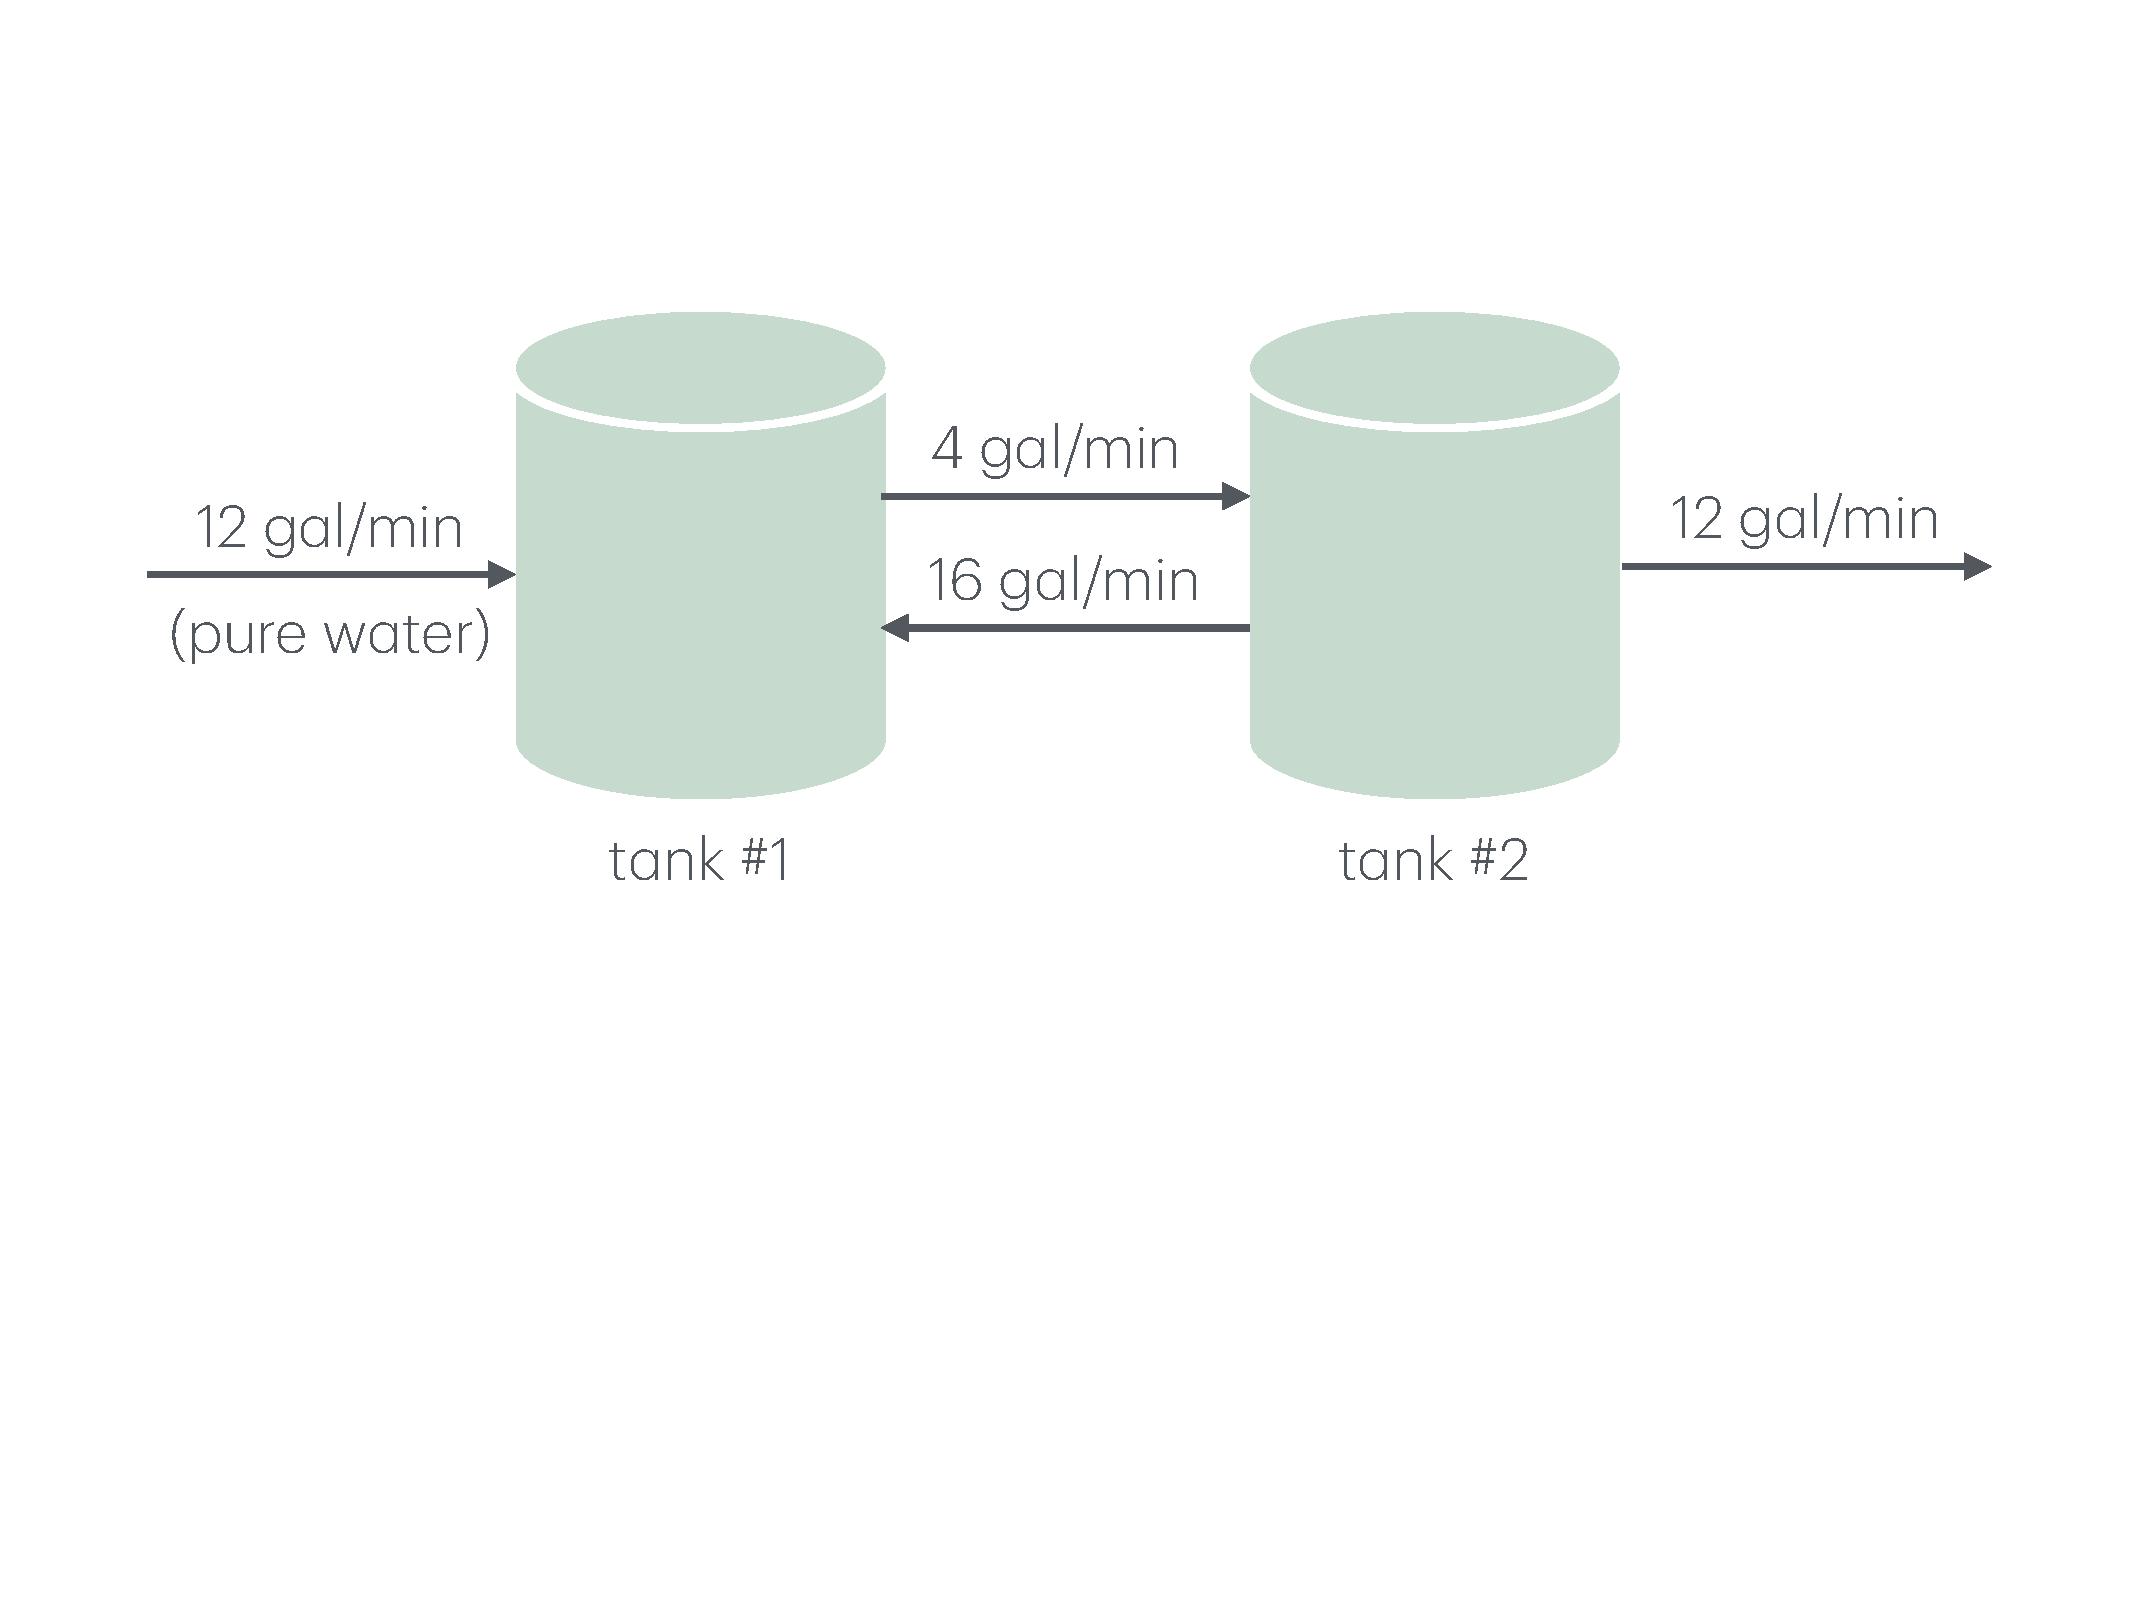
\includegraphics[width=0.8\linewidth]{tanks.pdf}

\begin{parts}
	\part set up a system of differential equations for $u_1(t)$ and $u_2(t)$, where $u_i(t)$ [lb/gal] is the concentration of fertilizer in tank $i \in \{1, 2\}$. write in matrix-vector form $\frac{d }{dt}[\mathbf{u}(t)]=A \mathbf{u}(t)$. don't forget the initial condition.
	
	\part compute the eigenvalues and eigenvectors of the coefficient matrix $A$ by hand.
	
	\part use the eigenvalues and eigenvectors of $A$ to write an expression for each $u_i(t)$ for $i\in \{1, 2\}$.
	
	\part plot the solutions $u_i(t)$ for $i\in \{1, 2\}$ ---for sufficiently long to see the steady-state behavior. does the behavior make sense?
\end{parts}

\subsection*{Markov chain}
% https://pubs.acs.org/doi/10.1021/ie900456j

\end{questions}
\end{document}
